
\chapter{统计与概率}
\section{矩的定义}
设 $x\in\mathbb R^{n}$ 是一个随机变量。
我们记 $m = E[x]\in\mathbb R^n$ 为期望，
记 $M=\mathrm{Var}[x] = E[(x-m)(x-m)^T]$ 为协方差（当这些量有定义时）。

在张量图中，我们会使用方括号：
\[
   \vecmatvec{1em}{}{}{m}
   =
\mathbin{\begin{tikzpicture}[baseline=(n0.base), inner sep=1pt]
   \node (n0) at (0,0) {$[$};
   \node [right=1em of n0] (n1) {$x]$};
   \draw (n0) -- (n1);
\end{tikzpicture}}
\quad\text{和}\quad
   \vecmatvec{1em}{}{M}{}
   =
\mathbin{\begin{tikzpicture}[baseline=(n0.base), inner sep=1pt]
   \node (n0) at (0,0) {$[$};
   \node [right=1em of n0] (n1) {$(x\ominus m)$};
   \node [right=.5em of n1] (n2) {$(x\ominus m)$};
   \node [right=1em of n2] (n3) {$]$};
   \draw (n0) -- (n1);
   \draw (n2) -- (n3);
\end{tikzpicture}}
\]
我们使用带圈减号 $\ominus$，以便把这个操作和缩并边区分开来。

我们还可以定义三阶和四阶中心矩张量：
\[
   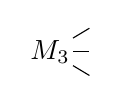
\begin{tikzpicture}[baseline=(T.base), inner sep=1pt]
      \node (T) {$M_3$};
      \draw (T) -- ++(.5,.3);
      \draw (T) -- ++(.5,-.3);
      \draw (T) -- ++(.5,0);
   \end{tikzpicture}
   =
   \renewcommand*{\arraystretch}{1.3}
   \begin{bmatrix}
      \vecmatvec{1em}{(x\ominus m)}{}{} \\
      \vecmatvec{1em}{(x\ominus m)}{}{} \\
      \vecmatvec{1em}{(x\ominus m)}{}{}
   \end{bmatrix}
\quad\text{和}\quad
   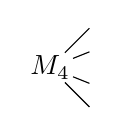
\begin{tikzpicture}[baseline=(T.base), inner sep=1pt]
      \node (T) {$M_4$};
      \draw (T) -- ++(.5,.5);
      \draw (T) -- ++(.5,-.5);
      \draw (T) -- ++(.5,.2);
      \draw (T) -- ++(.5,-.2);
   \end{tikzpicture}
   =
   \renewcommand*{\arraystretch}{1.3}
   \begin{bmatrix}
      \vecmatvec{1em}{(x\ominus m)}{}{} \\
      \vecmatvec{1em}{(x\ominus m)}{}{} \\
      \vecmatvec{1em}{(x\ominus m)}{}{} \\
      \vecmatvec{1em}{(x\ominus m)}{}{}
   \end{bmatrix}
.
\]
%These are less common in introductory causes, even though the scalar third and fourth moment are common.
%This is presumably because they require higher order tensors.

%If the entries of $x$ are independent, the non-diagonal entries disappear, so we get
%\[
%M =
%\left[
%   \begin{tikzpicture}[baseline=(c.base), inner sep=1pt]
%      \node (T1) {$(x\ominus m)$};
%      \node (T2)[below=.5em of T1] {$(x\ominus m)$};
%      \node (c)[right=.7em of T1, yshift=-1em] {$\sbullet$};
%      \draw (T1) -- (c);
%      \draw (T2) -- (c);
%      \draw (c) -- ++(.7em,0);
%   \end{tikzpicture}
%\right]
%\quad\text{and}\quad
%M_3 =
%\left[
%   \begin{tikzpicture}[baseline=(T2.base), inner sep=1pt]
%      \node (T1) {$(x\ominus m)$};
%      \node (T2)[below=.5em of T1] {$(x\ominus m)$};
%      \node (T3)[below=.5em of T2] {$(x\ominus m)$};
%      \node (c)[right=.7em of T2] {$\sbullet$};
%      \draw (T1) -- (c);
%      \draw (T2) -- (c);
%      \draw (T3) -- (c);
%      \draw (c) -- ++(.7em,0);
%   \end{tikzpicture}
%\right]
%\quad\text{and so on.}
%\]
% If the entries are also identically distributed, we simply have
% \[
%    M = \sigma^2
%    \,
% \begin{tikzpicture}[baseline=(T.base), inner sep=0]
%    \node (T) {$\sbullet$};
%    \draw (T) -- ++(0,.3);
%    \draw (T) -- ++(0,-.3);
% \end{tikzpicture}
%    \text{ and }
%    M_3 = \mathrm{E}[(x_0-m_0)^3]
% \begin{tikzpicture}[baseline=(T.base), inner sep=0]
%    \node (T) {$\sbullet$};
%    \draw (T) -- ++(0,.3);
%    \draw (T) -- ++(-.2,-.3);
%    \draw (T) -- ++(.2,-.3);
% \end{tikzpicture}
% .
% \]


\subsection{线性组合的期望}
一般原则：“期望的线性性”允许你把图中所有不涉及 $X$ 的部分提出去。
\[
   \vcenter{\hbox{
      \import{figures/}{linearityOfExpectation.pdf_tex}
   }}
\]
其中 $M_3$ 是期望\footnote{FIXME: 这与刚刚引入的记号不同。}
\(
\left[
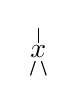
\begin{tikzpicture}[baseline=(T.base), inner sep=1pt]
   \node (T) {$x$};
   \draw (T) -- ++(0,.3);
   \draw (T) -- ++(-.1,-.3);
   \draw (T) -- ++(.1,-.3);
\end{tikzpicture}
\,
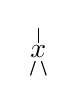
\begin{tikzpicture}[baseline=(T.base), inner sep=1pt]
   \node (T) {$x$};
   \draw (T) -- ++(0,.3);
   \draw (T) -- ++(-.1,-.3);
   \draw (T) -- ++(.1,-.3);
\end{tikzpicture}
\,
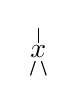
\begin{tikzpicture}[baseline=(T.base), inner sep=1pt]
   \node (T) {$x$};
   \draw (T) -- ++(0,.3);
   \draw (T) -- ++(-.1,-.3);
   \draw (T) -- ++(.1,-.3);
\end{tikzpicture}
\right]
\),
它是一个 9 阶张量，并且不依赖常量 $A$、$B$、$C$ 和 $D$。
在实践中，你会想给边命名，以便追踪哪些对象与哪些对象相乘。

我们甚至可以利用期望的线性性，把期望推进到张量的无穷和内部；如下矩生成函数把所有 $M_k$ 张量联系起来：
\begin{align*}
   \mathrm{E}(\mathrm{e}^{\langle x\ominus m, t\rangle})
   &= \sum_{k=0}^\infty \frac{1}{k!} \mathrm{E}[\langle x\ominus m, t\rangle^k]
    = \mathrm{E}\big[\sum_{k=0}^\infty \frac{1}{k!} \langle (x\ominus m)^{\otimes k}, t^{\otimes k}\rangle\big]
   = \sum_{k=0}^\infty \frac{1}{k!} \langle M_k, t^{\otimes k}\rangle
 \\&=
  % =
   1
   +
   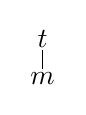
\begin{tikzpicture}[baseline=.5em, inner sep=1]
      \node (T) {$m$};
      \draw (T) -- ++(0,.5) node[fill=white] {$t$};
   \end{tikzpicture}
   +
   \frac{1}{2}
   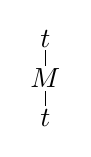
\begin{tikzpicture}[baseline=(T.base), inner sep=1]
      \node (T) {$M$};
      \draw (T) -- ++(0,.5) node[fill=white] {$t$};
      \draw (T) -- ++(0,-.5) node[fill=white] {$t$};
   \end{tikzpicture}
   +
   \frac{1}{6}
   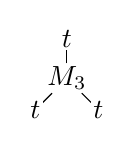
\begin{tikzpicture}[baseline=(T.base), inner sep=1]
      \node (T) {$M_3$};
      \draw (T) -- ++(0,.5) node[fill=white] {$t$};
      \draw (T) -- ++(-.4,-.4) node[fill=white] {$t$};
      \draw (T) -- ++(.4,-.4) node[fill=white] {$t$};
   \end{tikzpicture}
   +
   \frac{1}{24}
   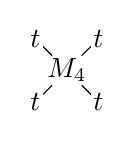
\begin{tikzpicture}[baseline=(T.base), inner sep=1]
      \node (T) {$M_4$};
      \draw (T) -- ++(-.4,-.4) node[fill=white] {$t$};
      \draw (T) -- ++(.4,-.4) node[fill=white] {$t$};
      \draw (T) -- ++(-.4,.4) node[fill=white] {$t$};
      \draw (T) -- ++(.4,.4) node[fill=white] {$t$};
   \end{tikzpicture}
   +
   \dots
\end{align*}

\subsection{线性形式}
《Matrix Cookbook》给出了下面这个简单的期望：
\begin{walign}
   \tag{312}
   \E[AXB+C] &= A \E[X] B + C
   &
   \renewcommand*{\arraystretch}{1.3}
   \begin{bmatrix}
      \matmul{A,X,B} \\+\, \matmul{C}
   \end{bmatrix}
   &=
   \renewcommand*{\arraystretch}{1.3}
   \begin{matrix}
      \matmul{A,[X],B} \\+\, \matmul{C}
   \end{matrix}
\end{walign}

\subsection{二次型}
我们常常更愿意用简单的中心矩来写期望；这可以通过提出均值来做到：
\renewcommand*{\arraystretch}{1}
\[
   \begin{bmatrix}
      x - \\
      x -
   \end{bmatrix}
   =
   \begin{bmatrix}
      (x\ominus m) - \\
      (x\ominus m) -
   \end{bmatrix}
   +
   \begin{array}{c}
      m - \\
      m -
   \end{array}
   =
   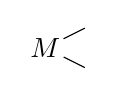
\begin{tikzpicture}[baseline=(T.base), inner sep=1pt]
      \node (T) {$M$};
      \draw (T) -- ++(.5,.25);
      \draw (T) -- ++(.5,-.25);
   \end{tikzpicture}
   +
   \begin{array}{c}
      m - \\
      m -
   \end{array}
\]
这样就很容易处理《Matrix Cookbook》中的二次型：
\begin{walign}
   \tag{313}
   \mathrm{Var}[Ax] &= A \mathrm{Var}[x] A^T
   &
   \renewcommand*{\arraystretch}{1.3}
   \begin{bmatrix}
      \vecmatvec{.5em}{A}{}{x} \ominus [\vecmatvec{.5em}{A}{}{x}] \\
      \vecmatvec{.5em}{A}{}{x} \ominus [\vecmatvec{.5em}{A}{}{x}]
   \end{bmatrix}
   &=
   \renewcommand*{\arraystretch}{1.3}
   \begin{bmatrix}
      \vecmatvec{.5em}{A}{}{(x\ominus m)} \\
      \vecmatvec{.5em}{A}{}{(x\ominus m)}
   \end{bmatrix}
 \\&&&=
   \vcenter{\hbox{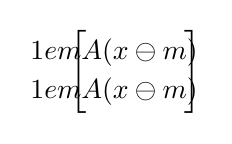
\begin{tikzpicture}[inner sep=1pt]
      \node (n1) at (0,-.25) {$\vecmatvec{1em}{A}{}{(x\ominus m)}$};
      \node (n2) at (0,.25) {$\vecmatvec{1em}{A}{}{(x\ominus m)}$};
      \node at (-.45, 0) {$\Bigg[$};
      \node at (1, 0) {$\Bigg]$};
   \end{tikzpicture}}}
 \\&&& =
   \vecmatvec{.5em}{}{A,M_2,A}{}
%%%%%%%%%%%%%%%%%%%%%%%%%%%%%%%%%%%%%%%%%%%%%%%%%%%%%%%%%%%%%%%%%%%%%%%%%%%%%%%%
   \\[.5em]
   \tag{318}
   \E[x^T A x]
   &= \mathrm{Tr}(A M) + m^T A m
   &
   [\vecmatvec{.5em}{x}{A}{x}]
   &=
   \left(
      \begin{bmatrix}
         (x\ominus m) - \\
         (x\ominus m) -
      \end{bmatrix}
      +
      \begin{array}{c}
         m - \\
         m -
      \end{array}
   \right)
   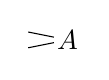
\begin{tikzpicture}[baseline=(A.base), inner sep=1pt]
      \node (A) {$A$};
      \draw (A) -- ++(-.5, .1);
      \draw (A) -- ++(-.5, -.1);
   \end{tikzpicture}
   \\
   &&&=
   \mathbin{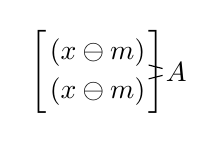
\begin{tikzpicture}[baseline=(A.base), inner sep=1pt]
      \node (n1) at (0,-.25) {$(x\ominus m)$};
      \node (n2) at (0,.25) {$(x\ominus m)$};
      \node at (-.75, 0) {$\Bigg[$};
      \node at (.75, 0) {$\Bigg]$};
      \node (A) at (1, 0) {$A$};
      \draw (n1) -- (A);
      \draw (n2) -- (A);
   \end{tikzpicture}}
   +
   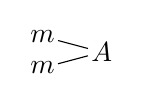
\begin{tikzpicture}[baseline=(A.base), inner sep=1pt]
      \node (A) {$A$};
      \node (m1) at (-.75, .2) {$m$};
      \node (m2) at (-.75, -.2) {$m$};
      \draw (m1) -- (A) -- (m2);
   \end{tikzpicture}
   \\
   &&&=
   \trace{M,A}2
   +
   \vecmatvec{.5em}{m}{A}{m}
   \\[.5em]
\end{walign}

\begin{align*}
   E[(A\mathbf{x} + a)(B\mathbf{x} + b)^T] &= AMB^T + (Am + a)(Bm + b)^T \tag{320} \\
   E[\mathbf{x}\mathbf{x}^T] &= M + mm^T \tag{321} \\
   E[\mathbf{x} a^T \mathbf{x}] &= (M + mm^T)a \tag{322} \\
   E[\mathbf{x}^T a\mathbf{x}^T] &= a^T(M + mm^T) \tag{323} \\
   E[(A\mathbf{x})(A\mathbf{x})^T] &= A(M + mm^T)A^T \tag{324} \\
   E[(\mathbf{x} + a)(\mathbf{x} + a)^T] &= M + (m + a)(m + a)^T \tag{325} \\
   E[(A\mathbf{x} + a)^T(B\mathbf{x} + b)] &= \text{Tr}(AMB^T) + (Am + a)^T(Bm + b) \tag{326} \\
   E[\mathbf{x}^T \mathbf{x}] &= \text{Tr}(M) + m^T m \tag{327} \\
   E[\mathbf{x}^T A\mathbf{x}] &= \text{Tr}(AM) + m^T Am \tag{328} \\
   E[(A\mathbf{x})^T(A\mathbf{x})] &= \text{Tr}(AMA^T) + (Am)^T(Am) \tag{329} \\
   E[(\mathbf{x} + a)^T(\mathbf{x} + a)] &= \text{Tr}(M) + (m + a)^T(m + a) \tag{330}
\end{align*}



\subsection{三次型}

\[
\begin{tikzpicture}[scale=1.3,
  every node/.style={inner sep=1pt, circle, draw, fill=white, thin},
  label/.style={draw=none, fill=none, text=black, font=\scriptsize},
  declare function={
    xgap=.8;  % Horizontal spacing between diagrams
  }]

  \drawPartitionAtAngle{(-1.6*xgap,0)}{3}{$\kappa_3$}{{{1,2,3}}}
  \drawPartitionAtAngle{(0,0)}{3}{$+\kappa_2\kappa_1\Big($}{{{1,2},{3}}}
  \drawPartitionAtAngle{(xgap,0)}{3}{$+$}{{{1,3},{2}}}
  \drawPartitionAtAngle{(2*xgap,0)}{3}{$+$}{{{2,3},{1}}}
  \drawPartitionAtAngle{(3.6*xgap,0)}{3}{$\Big)+\kappa_1^3$}{{{1},{2},{3}}}

\end{tikzpicture}
\]


当 $x$ 是均值向量为 $m$ 的随机向量时，
把原始三阶矩展开为中心矩会很方便：

\renewcommand*{\arraystretch}{1}
\begin{align*}
\begin{bmatrix}
   x - \\
   x - \\
   x -
\end{bmatrix}
&=
\begin{bmatrix}
   (x\ominus m) - \\
   (x\ominus m) - \\
   (x\ominus m) -
\end{bmatrix}
\vspace{-.5em}
+
3
\hspace{-.25em}
\begin{array}{l}
\begin{bmatrix}
   (x\ominus m) -
\end{bmatrix}\\[.1em]
\begin{bmatrix}
   m - \\
   m -
\end{bmatrix}
\end{array}
\hspace{-.5em}
+
3
\hspace{-.25em}
\begin{array}{l}
\begin{bmatrix}
   m -
\end{bmatrix}\\[.1em]
\begin{bmatrix}
   (x\ominus m) - \\
   (x\ominus m) -
\end{bmatrix}
\end{array}
\hspace{-.5em}
+
\hspace{-.5em}
\begin{array}{c}
\begin{bmatrix}
   m -
\end{bmatrix}\\[.1em]
\begin{bmatrix}
   m -
\end{bmatrix}\\[.1em]
\begin{bmatrix}
   m -
\end{bmatrix}
\end{array}
%
\\&=
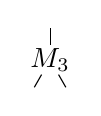
\begin{tikzpicture}[baseline=(T.base), inner sep=1pt]
   \node (T) {$M_3$};
   \draw (T) -- ++(0,.4);
   \draw (T) -- ++(-.2,-.35);
   \draw (T) -- ++(.2,-.35);
\end{tikzpicture}
+
3
\hspace{-.25em}
\begin{array}{c}
   m - \\
   -M-
\end{array}
\hspace{-.5em}
+
\begin{array}{c}
   m - \\
   m - \\
   m -
\end{array}
\end{align*}
TODO: $m,M$ 项中的边需要做对称化。


但这仍然有些杂乱。
另见下面关于累积量的内容。



假设 \(\mathbf{x}\) 是一个坐标相互独立的随机向量，均值为 \(m\)，
协方差为 \(M\)，中心矩为 \(v_3 = \mathbb{E}[(\mathbf{x} - m)^3]\)。那么（见 [7]）
\begin{align*}
&\mathbb{E}[(A\mathbf{x} + a)(B\mathbf{x} + b)^T (C\mathbf{x} + c)]
\\&\quad=
A\,\mathrm{diag}(B^T C) v_3
\\&\quad+
(Am + a) \mathrm{Tr}(BMC^T)
\\&\quad+
AMC^T (Bm + b)
\\&\quad\,+
AMB^T (Cm + c)
\\&\quad+
(Am + a)(Bm + b)^T (Cm + c)
\\
  &\mathbb{E}[\mathbf{x} \mathbf{x}^T \mathbf{x}]
\\&\quad=
   v_3
\\&\quad+
   2 Mm
\\&\quad+
   (\text{Tr}(M) + m^T m) m
\end{align*}


\section{累积量}

给定随机向量 $x\in\mathbb R^d$，
它的 $n$ 阶累积量张量 $K_n\in\R^{d,\ldots,d}$ 定义为
\[
   \log \mathrm{E}(\mathrm{e}^{\langle t, x\rangle})
   = \sum_{n=1}^\infty \frac{1}{n!} \langle K_n, t^{\otimes n}\rangle
   =
   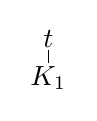
\begin{tikzpicture}[baseline=.5em, inner sep=1]
      \node (T) {$K_1$};
      \draw (T) -- ++(0,.5) node[fill=white] {$t$};
   \end{tikzpicture}
   +
   \frac{1}{2}
   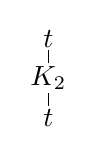
\begin{tikzpicture}[baseline=(T.base), inner sep=1]
      \node (T) {$K_2$};
      \draw (T) -- ++(0,.5) node[fill=white] {$t$};
      \draw (T) -- ++(0,-.5) node[fill=white] {$t$};
   \end{tikzpicture}
   +
   \frac{1}{6}
   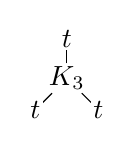
\begin{tikzpicture}[baseline=(T.base), inner sep=1]
      \node (T) {$K_3$};
      \draw (T) -- ++(0,.5) node[fill=white] {$t$};
      \draw (T) -- ++(-.4,-.4) node[fill=white] {$t$};
      \draw (T) -- ++(.4,-.4) node[fill=white] {$t$};
   \end{tikzpicture}
   +
   \dots
\]
前几个累积量类似于中心矩：
\[
   K_1 = m
   \quad\text{和}\quad
   K_2 = M
   \quad\text{和}\quad
   K_3 = M_3
   \quad\text{和}\quad
   K_4 = M_4
   - \begin{tikzpicture}[baseline=-.8em, inner sep=.5pt]
      \node (M1) {\scriptsize $M_2$};
      \node[below=.4em of M1] (M2) {\scriptsize $M_2$};
      \draw (M1) -- ++(.35,0);
      \draw (M2) -- ++(.35,0);
      \draw (M1) -- ++(-.35,0);
      \draw (M2) -- ++(-.35,0);
   \end{tikzpicture}
   - \begin{tikzpicture}[baseline=(M1.base), inner sep=.5pt]
      \node (M1) {\scriptsize $M_2$};
      \node[right=.05em of M1] (M2) {\scriptsize $M_2$};
      \draw (M1) -- ++(-.25,.25);
      \draw (M1) -- ++(-.25,-.25);
      \draw (M2) -- ++(.25,.25);
      \draw (M2) -- ++(.25,-.25);
   \end{tikzpicture}
   - \begin{tikzpicture}[baseline=(M1.base), inner sep=.5pt]
      \node (M1) {\scriptsize $M_2$};
      \node[right=.05em of M1, yshift=-2pt] (M2) {\scriptsize $M_2$};
      \draw (M1) -- ++(-.25,.25);
      \draw (M1) -- ++(+.7,-.25);
      \draw (M2) -- ++(-.7,-.25);
      \draw (M2) -- ++(.25,.25);
   \end{tikzpicture}
   .
\]
它们有一个很好的性质（从定义很容易看出）：对于独立随机变量，累积量是可加的：
$
   K_n(x + y) = K_n(x) + K_n(y).
$
这推广了一个标准性质：独立随机变量之和的方差等于方差之和。

我们可以用累积量来写出 $x^{\otimes n}$ 的期望：

\[
   \begin{bmatrix}
      \begin{tikzpicture}[
         baseline=(T.base),
         every node/.style={inner sep=1pt, circle, draw=none, fill=white},
       ]
       \draw (30:.2) node[label] {$x$} -- (30:.6);
       \draw (150:.2) node[label] {$x$} -- (150:.6);
       \draw (270:.2) node[label] {$x$} -- (270:.6);
      \end{tikzpicture}
   \end{bmatrix}
   =
   \begin{tikzpicture}[
      baseline=-1em,
     every node/.style={inner sep=1pt, circle, draw, fill=white, thin},
     label/.style={draw=none, fill=none, text=black, font=\scriptsize},
     declare function={
       xgap=1.8;  % Horizontal spacing between diagrams
     }]
     \drawPartitionAtAngle[k]{(-1*xgap,0)}{3}{}{{{1,2,3}}}
     \drawPartitionAtAngle[k]{(0,0)}{3}{$+$}{{{1,2},{3}}}
     \drawPartitionAtAngle[k]{(xgap,0)}{3}{$+$}{{{1,3},{2}}}
     \drawPartitionAtAngle[k]{(xgap*2,0)}{3}{$+$}{{{1},{2,3}}}
     \drawPartitionAtAngle[k]{(xgap*3,0)}{3}{$+$}{{{1},{2},{3}}}
   \end{tikzpicture}
   .
\]
一般而言，求和遍历集合 $\{1,\ldots,n\}$ 的所有划分。

如果 $x$ 的各个分量\emph{相互独立}，累积量张量 $K_1, K_2, \dots$ 的非对角项为零。
这意味着可以按如下方式写出：
%
假设每个 $x_i$ 的累积量为 $\kappa_1, \kappa_2, \kappa_3, \kappa_4 \in \R$，则
\[
\begin{bmatrix}
   \begin{tikzpicture}[
      baseline=(T.base),
      every node/.style={inner sep=1pt, circle, draw=none, fill=white},
    ]
    \draw (30:.2) node[label] {$x$} -- (30:.5);
    \draw (120:.2) node[label] {$x$} -- (120:.5);
    \draw (210:.2) node[label] {$x$} -- (210:.5);
    \draw (300:.2) node[label] {$x$} -- (300:.5);
   \end{tikzpicture}
\end{bmatrix}
=
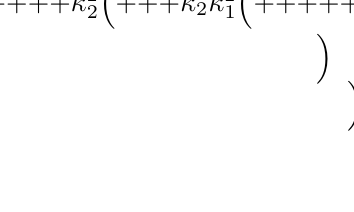
\begin{tikzpicture}[
  every node/.style={inner sep=1pt, circle, draw, fill=white, thin},
  label/.style={draw=none, fill=none, text=black, font=\scriptsize},
  declare function={
    xgap=1;  % Horizontal spacing between diagrams
    ygap=.6;  % Vertical spacing between rows
  },
  baseline=-1cm
  ]
  \pgfmathsetmacro{\outerRadius}{.3}
  \pgfmathsetmacro{\innerRadius}{.1}

  % Pattern {4} - 1 partition
  \drawPartitionAtAngle{(0,0)}{4}{$\kappa_4$}{{{1,2,3,4}}}

  % Pattern {3,1} - 4 partitions
  \drawPartitionAtAngle{(0,-ygap)}{4}{$+\kappa_3\kappa_1\Big($}{{{1,2,3},{4}}}
  \drawPartitionAtAngle{(xgap,-ygap)}{4}{$+$}{{{1,2,4},{3}}}
  \drawPartitionAtAngle{(2*xgap,-ygap)}{4}{$+$}{{{2},{1,3,4}}}
  \drawPartitionAtAngle{(3*xgap,-ygap)}{4}{$+$}{{{1},{2,3,4}}}
  \node[label] at (3.5*xgap,-ygap) {$\Big)$};

  % Pattern {2,2} - 3 partitions
  \drawPartitionAtAngle{(0,-2*ygap)}{4}{$+\kappa_2^2\Big($}{{{1,2},{3,4}}}
  \drawPartitionAtAngle{(xgap,-2*ygap)}{4}{$+$}{{{1,3},{2,4}}}
  \drawPartitionAtAngle{(2*xgap,-2*ygap)}{4}{$+$}{{{1,4},{2,3}}}
  \node[label] at (2.5*xgap,-2*ygap) {$\Big)$};

  % Pattern {2,1,1} - 6 partitions
  \drawPartitionAtAngle{(0,-3*ygap)}{4}{$+\kappa_2\kappa_1^2\Big($}{{{1,2},{3},{4}}}
  \drawPartitionAtAngle{(xgap,-3*ygap)}{4}{$+$}{{{1,3},{2},{4}}}
  \drawPartitionAtAngle{(2*xgap,-3*ygap)}{4}{$+$}{{{1,4},{2},{3}}}
  \drawPartitionAtAngle{(3*xgap,-3*ygap)}{4}{$+$}{{{1},{2,3},{4}}}
  \drawPartitionAtAngle{(4*xgap,-3*ygap)}{4}{$+$}{{{1},{3},{2,4}}}
  \drawPartitionAtAngle{(5*xgap,-3*ygap)}{4}{$+$}{{{1},{2},{3,4}}}
  \node[label] at (5.5*xgap,-3*ygap) {$\Big)$};

  % Pattern {1,1,1,1} - 1 partition
  \drawPartitionAtAngle{(0,-4*ygap)}{4}{$+\kappa_1^4$}{{{1},{2},{3},{4}}}

\end{tikzpicture}
\]

特别注意，如果均值 $\kappa_1$ 为零，就只剩下四项。
%\(
%\begin{tikzpicture}[
%   baseline=4em,
%  every node/.style={inner sep=1pt, circle, draw, fill=white, thin},
%  label/.style={draw=none, fill=none, text=black, font=\scriptsize},
%  declare function={
%    xgap=1;  % Horizontal spacing between diagrams
%    ygap=.6;  % Vertical spacing between rows
%  },
%  baseline=-1cm
%  ]
%  \pgfmathsetmacro{\outerRadius}{.3}
%  \pgfmathsetmacro{\innerRadius}{.1}
%
%  \drawPartitionAtAngle{(-1.5*xgap,0)}{4}{$\kappa_4$}{{{1,2,3,4}}}
%  \drawPartitionAtAngle{(0,0)}{4}{$+\kappa_2^2\Big($}{{{1,2},{3,4}}}
%  \drawPartitionAtAngle{(xgap,0)}{4}{$+$}{{{1,3},{2,4}}}
%  \drawPartitionAtAngle{(2*xgap,0)}{4}{$+$}{{{1,4},{2,3}}}
%  \node[label] at (2.5*xgap,0) {$\Big)$};
%\end{tikzpicture}
%.
%\)
当 $n=5$ 时，总共有 52 个划分；但若 $\kappa_1=0$，只有 11 项保留下来：
\[
   \begin{tikzpicture}[
     every node/.style={inner sep=1pt, circle, draw, fill=white, thin},
     label/.style={draw=none, fill=none, text=black, font=\scriptsize},
     declare function={
       xgap=1;  % Horizontal spacing between diagrams
       ygap=.6;  % Vertical spacing between rows
     },
     baseline=-1cm
     ]
     \pgfmathsetmacro{\outerRadius}{.3}
     \pgfmathsetmacro{\innerRadius}{.1}
   % Pattern {5} - 1 partition
   \drawPartitionAtAngle{(-1.8*xgap,-ygap)}{5}{$\kappa_5$}{{{1,2,3,4,5}}}
   % Pattern {3,2} - 10 partitions
   \drawPartitionAtAngle{(0,-ygap)}{5}{$+\kappa_3\kappa_2\Big($}{{{1,2,3},{4,5}}}
   \drawPartitionAtAngle{(xgap,-ygap)}{5}{$+$}{{{3,5},{1,2,4}}}
   \drawPartitionAtAngle{(2*xgap,-ygap)}{5}{$+$}{{{1,2,5},{3,4}}}
   \drawPartitionAtAngle{(3*xgap,-ygap)}{5}{$+$}{{{1,3,4},{2,5}}}
   \drawPartitionAtAngle{(4*xgap,-ygap)}{5}{$+$}{{{1,3,5},{2,4}}}
   \drawPartitionAtAngle{(5*xgap,-ygap)}{5}{$+$}{{{1,4,5},{2,3}}}
   \drawPartitionAtAngle{(6*xgap,-ygap)}{5}{$+$}{{{1,5},{2,3,4}}}
   \drawPartitionAtAngle{(7*xgap,-ygap)}{5}{$+$}{{{2,3,5},{1,4}}}
   \drawPartitionAtAngle{(8*xgap,-ygap)}{5}{$+$}{{{1,3},{2,4,5}}}
   \drawPartitionAtAngle{(9*xgap,-ygap)}{5}{$+$}{{{1,2},{3,4,5}}}
   \node[label] at (9.5*xgap,-ygap) {$\Big)$};
   \end{tikzpicture}
\]

如果 $x$ 是高斯变量，所有 3 阶及更高阶累积量都为零。
当 $n=6$ 时，总共有 203 个划分，但 $E[x^{\otimes 6}]$ 只剩 15 项\footnote{这就是为什么对 $g\sim N(0,1)$ 有 $\E[g^6]=15$。}：
\[
   \begin{tikzpicture}[
     every node/.style={inner sep=1pt, circle, draw, fill=white, thin},
     label/.style={draw=none, fill=none, text=black, font=\scriptsize},
     declare function={
       xgap=1;  % Horizontal spacing between diagrams
       ygap=.8;  % Vertical spacing between rows
     },
     baseline=-1cm
     ]
     \pgfmathsetmacro{\outerRadius}{.3}
     \pgfmathsetmacro{\innerRadius}{.1}
     % Pattern {2,2,2} - 15 partitions
     \drawPartitionAtAngle{(0,0)}{6}{$\kappa_2^3\Big($}{{{1,2},{3,4},{5,6}}}
     \drawPartitionAtAngle{(xgap,0)}{6}{$+$}{{{1,2},{3,5},{4,6}}}
     \drawPartitionAtAngle{(2*xgap,0)}{6}{$+$}{{{1,2},{3,6},{4,5}}}
     \drawPartitionAtAngle{(3*xgap,0)}{6}{$+$}{{{1,3},{2,4},{5,6}}}
     \drawPartitionAtAngle{(4*xgap,0)}{6}{$+$}{{{1,3},{2,5},{4,6}}}
     \drawPartitionAtAngle{(5*xgap,0)}{6}{$+$}{{{1,3},{2,6},{4,5}}}
     \drawPartitionAtAngle{(6*xgap,0)}{6}{$+$}{{{1,4},{2,3},{5,6}}}
     % row 2
     \drawPartitionAtAngle{(1*xgap,-ygap)}{6}{$+$}{{{1,4},{2,5},{3,6}}}
     \drawPartitionAtAngle{(2*xgap,-ygap)}{6}{$+$}{{{1,4},{2,6},{3,5}}}
     \drawPartitionAtAngle{(3*xgap,-ygap)}{6}{$+$}{{{1,5},{2,3},{4,6}}}
     \drawPartitionAtAngle{(4*xgap,-ygap)}{6}{$+$}{{{1,5},{2,4},{3,6}}}
     \drawPartitionAtAngle{(5*xgap,-ygap)}{6}{$+$}{{{1,5},{2,6},{3,4}}}
     \drawPartitionAtAngle{(6*xgap,-ygap)}{6}{$+$}{{{1,6},{2,3},{4,5}}}
     \drawPartitionAtAngle{(7*xgap,-ygap)}{6}{$+$}{{{1,6},{3,5},{2,4}}}
     \drawPartitionAtAngle{(8*xgap,-ygap)}{6}{$+$}{{{1,6},{3,4},{2,5}}}
     \node[label] at (8.5*xgap,-ygap) {$\Big)$};
     \end{tikzpicture}
     .
\]

\subsection{四次型}





我们可以用它来计算 $\mathrm{Var}[x^T A x]$。
假设 $A$ 是对称的：
\begin{walign}
   \mathrm{Var}[x^T A x]
   &=
   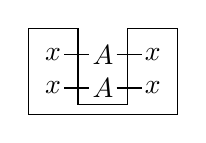
\begin{tikzpicture}[baseline=.5em, inner sep=1pt, x=1.8em, y=1.2em]
      \node (x0) at (0,0) {$x$};
      \node (A0) at (1,0) {$A$};
      \node (x1) at (2,0) {$x$};
      \draw (x0) -- (A0) -- (x1);
      \node (x2) at (0,1) {$x$};
      \node (A1) at (1,1) {$A$};
      \node (x3) at (2,1) {$x$};
      \draw (x2) -- (A1) -- (x3);
      \draw (-.5,-.8) -- (2.5,-.8) -- (2.5,1.8) -- (1.5,1.8) -- (1.5,-.5) -- (.5,-.5) -- (.5,1.8) -- (-.5,1.8) -- (-.5,-.8);
   \end{tikzpicture}
   -
   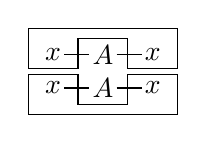
\begin{tikzpicture}[baseline=.5em, inner sep=1pt, x=1.8em, y=1.2em]
      \node (x0) at (0,0) {$x$};
      \node (A0) at (1,0) {$A$};
      \node (x1) at (2,0) {$x$};
      \draw (x0) -- (A0) -- (x1);
      \node (x2) at (0,1) {$x$};
      \node (A1) at (1,1) {$A$};
      \node (x3) at (2,1) {$x$};
      \draw (x2) -- (A1) -- (x3);
      \draw (-.5,-.8) -- (2.5,-.8) -- (2.5,.4) -- (1.5,.4) -- (1.5,-.5) -- (.5,-.5) -- (.5,.4) -- (-.5,.4) -- (-.5,-.8);
      \draw (-.5,1.8) -- (2.5,1.8) -- (2.5,.6) -- (1.5,.6) -- (1.5,1.5) -- (.5,1.5) -- (.5,.6) -- (-.5,.6) -- (-.5,1.8);
   \end{tikzpicture}
   \\&=
   \kappa_4
   \begin{tikzpicture}[baseline=(A0.base), inner sep=0pt, fill=white]
       \node (A1) at (0,0) {$A$};
       \node (bullet) at (.8,0) {$\sbullet$};
       \node[anchor=west] (A2) at (1.4,0) {$A$};
       \draw (A1.east) to[out=45,in=135] (bullet) to[out=45,in=135] (A2.west);
       \draw (A1.east) to[out=-45,in=-135] (bullet) to[out=-45,in=-135] (A2.west);
   \end{tikzpicture}
   +
   4\kappa_3\kappa_1
   \begin{tikzpicture}[baseline=(A0.base), inner sep=1pt]
       \node (A1) at (0,0) {$A$};
       \node (bullet) at (.8,0) {$\sbullet$};
       \node[anchor=west] (A2) at (1.1,0) {$A$};
       \node (bullet2) at (1.8,0) {$\sbullet$};
       \draw (A1.east) to[out=45,in=135] (bullet) -- (A2.west);
       \draw (A1.east) to[out=-45,in=-135] (bullet);
       \draw (A2.east) -- (bullet2);
   \end{tikzpicture}
   \\&\quad+
   2 \kappa_2^2 \hspace{-.5em}\trace{A,A}{2}\hspace{-.5em} + \kappa_2^2 \hspace{-1em}\trace{A}{1}\hspace{-2em}\trace{A}{1}
   \\&\quad+
   4\kappa_2\kappa_1^2
   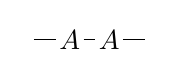
\begin{tikzpicture}[baseline=(A.base), inner sep=1pt]
       \node (bullet) at (0,0) {$\sbullet$};
       \node (A) at (.5,0) {$A$};
       \node (A2) at (1,0) {$A$};
       \node (bullet2) at (1.5,0) {$\sbullet$};
       \draw (bullet.east) -- (A.west);
       \draw (A.east) -- (A2.west);
       \draw (A2.east) -- (bullet2.west);
   \end{tikzpicture}
   +2\kappa_2\kappa_1^2
   \hspace{-1em} \trace{A}{1}\hspace{-1em}
   \vecmatvec{.5em}{\sbullet}{A}{\sbullet}
   \\&\quad+\kappa_1^4 \vecmatvec{.5em}{\sbullet}{A}{\sbullet}
   \vecmatvec{.5em}{\sbullet}{A}{\sbullet}
   \\&\quad-\big(
      \kappa_2 
      \hspace{-1em} \trace{A}{1}\hspace{-1em}
      +
      \kappa_1^2
      \vecmatvec{.5em}{\sbullet}{A}{\sbullet}
   \big)^2
   \\&=
   %%%
   2 \kappa_2^2 \hspace{-.5em}\trace{A,A}{2}\hspace{-.5em}
   +4\kappa_2\kappa_1^2
   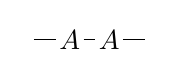
\begin{tikzpicture}[baseline=(A.base), inner sep=1pt]
       \node (bullet) at (0,0) {$\sbullet$};
       \node (A) at (.5,0) {$A$};
       \node (A2) at (1,0) {$A$};
       \node (bullet2) at (1.5,0) {$\sbullet$};
       \draw (bullet.east) -- (A.west);
       \draw (A.east) -- (A2.west);
       \draw (A2.east) -- (bullet2.west);
   \end{tikzpicture}
   \\&\quad+
   4\kappa_3\kappa_1
   \begin{tikzpicture}[baseline=(A0.base), inner sep=1pt]
       \node (A1) at (0,0) {$A$};
       \node (bullet) at (.8,0) {$\sbullet$};
       \node[anchor=west] (A2) at (1.1,0) {$A$};
       \node (bullet2) at (1.8,0) {$\sbullet$};
       \draw (A1.east) to[out=45,in=135] (bullet) -- (A2.west);
       \draw (A1.east) to[out=-45,in=-135] (bullet);
       \draw (A2.east) -- (bullet2);
   \end{tikzpicture}
   +\kappa_4
   \begin{tikzpicture}[baseline=(A0.base), inner sep=0pt, fill=white]
       \node (A1) at (0,0) {$A$};
       \node (bullet) at (.8,0) {$\sbullet$};
       \node[anchor=west] (A2) at (1.4,0) {$A$};
       \draw (A1.east) to[out=45,in=135] (bullet) to[out=45,in=135] (A2.west);
       \draw (A1.east) to[out=-45,in=-135] (bullet) to[out=-45,in=-135] (A2.west);
   \end{tikzpicture}
\end{walign}
《Matrix Cookbook》把它列为
\[
   \mathrm{Var}[x^T A x]
   =
   2\mu_2^2\text{Tr}(A^2)
   + 4\mu_2 c^T A^2 c
   + 4\mu_3 c^T Aa
   + (\mu_4 - 3\mu_2^2)a^T a \tag{319}
\]
其中 $c = \mu_1$ 是 $x$ 的均值，
$a = \mathrm{diag}(A)$ 是 $A$ 的对角线，
而 $\mu_4 = \kappa_4 + 3\kappa_2^2$ 是四阶中心矩。


\section{加权标量变量}
令 $y=w^T x$，并令 $m=E[y]$，则
\begin{align*}
   \tag{321}
   \E[y] &= m = w^T \mu
   \\
   \tag{322}
   \E[(y\ominus m)^2] &= \vecmatvec{.5em}{w}{M_2}{w}
   \\
   \tag{323}
   \E[(y\ominus m)^3] &=
   \mathbin{\begin{tikzpicture}[baseline=(a0.base), inner sep=1pt]
      \node (a0) {$M_3$};
      \node[above=.3em of a0] (n0) {$w$};
      \node[right=.3em of a0] (n1) {$w$};
      \node[left=.3em of a0] (n3) {$w$};
      \draw (a0.north) -- (n0);
      \draw (a0.east) -- (n1);
      \draw (a0.west) -- (n3);
   \end{tikzpicture}}
   \\
   \tag{324}
   \E[(y\ominus m)^4] &=
   \mathbin{\begin{tikzpicture}[baseline=(a0.base), inner sep=1pt]
      \node (a0) {$M_4$};
      \node[above=.3em of a0] (n0) {$w$};
      \node[right=.3em of a0] (n1) {$w$};
      \node[below=.3em of a0] (n2) {$w$};
      \node[left=.3em of a0] (n3) {$w$};
      \draw (a0.north) -- (n0);
      \draw (a0.east) -- (n1);
      \draw (a0.south) -- (n2);
      \draw (a0.west) -- (n3);
   \end{tikzpicture}}
\end{align*}


对于 $x\sim N(0,1)$，有不等式：
\[
   \E[y^n]^{1/n} \leq \sqrt{2/\pi}\, \|w\|_2.
\]


\section{高斯矩}

对于高斯向量 $x \sim \mathcal{N}(m,M)$：
- 所有奇数阶中心矩都为零：$M_3 = 0$，等等。
- 偶数阶矩可以通过 Isserlis 定理计算。

例如：
\[
\mathbb{E}[(x \ominus m)^{\otimes 4}]
=
M \otimes M + M \otimes M + \dots
\]
（对指标的不同配对求和）。

\subsection{高斯分部积分}
如果 $X$ 是一个由高斯条目组成、均值为零且带有某个协方差的张量，
% General principle for Gaussian expectations.
那么对任意可微函数 $f$，Stein 引理给出下面这个非常一般的方程：
\[
   \vcenter{\hbox{
      \import{figures/}{steins.pdf_tex}
   }}
\]
结合第~\ref{chapter:functions} 章中的张量链式法则，这可以成为求解许多困难期望的强大方法。



\begin{align*}
E(xx^T) &= \Sigma + mm^T \tag{377} \\
E[x^TAx] &= \text{Tr}(A\Sigma) + m^TAm \tag{378} \\
\text{Var}(x^TAx) &= \text{Tr}[A\Sigma(A + A^T)\Sigma] + \cdots \tag{379} \\
&\quad +m^T(A + A^T)\Sigma(A + A^T)m \\
E[(x - m')^TA(x - m')] &= (m - m')^TA(m - m') + \text{Tr}(A\Sigma) \tag{380}
\end{align*}

如果 $\Sigma = \sigma^2I$ 且 $A$ 对称，则

\begin{align*}
\text{Var}(x^TAx) = 2\sigma^4\text{Tr}(A^2) + 4\sigma^2m^TA^2m \tag{381}
\end{align*}

假设 $x \sim \mathcal{N}(0, \sigma^2I)$，且 $A$ 和 $B$ 对称，则

\begin{align*}
\text{Cov}(x^TAx, x^TBx) = 2\sigma^4\text{Tr}(AB) \tag{382}
\end{align*}

\subsection{三次型}

假设 $x$ 是一个坐标相互独立的随机向量，均值为 $m$，协方差为 $M$：

\begin{align*}
E[xb^Txx^T] &= mb^T(M + mm^T) + (M + mm^T)bm^T \tag{383} \\
&\quad +b^Tm(M - mm^T)
\end{align*}

\subsection{四次型的均值}

\begin{align*}
E[xx^Txx^T] &= 2(\Sigma + mm^T)^2 + m^Tm(\Sigma - mm^T) \\
&\quad +\text{Tr}(\Sigma)(\Sigma + mm^T) \\[1em]
E[xx^TAxx^T] &= (\Sigma + mm^T)(A + A^T)(\Sigma + mm^T) \\
&\quad +m^TAm(\Sigma - mm^T) + \text{Tr}[A\Sigma](\Sigma + mm^T) \\[1em]
E[x^Txx^Tx] &= 2\text{Tr}(\Sigma^2) + 4m^T\Sigma m + (\text{Tr}(\Sigma) + m^Tm)^2 \\[1em]
E[x^TAxx^TBx] &= \text{Tr}[A\Sigma(B + B^T)\Sigma] + m^T(A + A^T)\Sigma(B + B^T)m \\
&\quad +(\text{Tr}(A\Sigma) + m^TAm)(\text{Tr}(B\Sigma) + m^TBm)
\end{align*}

\begin{align*}
E[a^Txb^Txc^Txd^Tx] &= (a^T(\Sigma + mm^T)b)(c^T(\Sigma + mm^T)d) \\
&\quad +(a^T(\Sigma + mm^T)c)(b^T(\Sigma + mm^T)d) \\
&\quad +(a^T(\Sigma + mm^T)d)(b^T(\Sigma + mm^T)c) - 2a^Tmb^Tmc^Tmd^Tm
\end{align*}

\begin{align*}
&E[(Ax + a)(Bx + b)^T(Cx + c)(Dx + d)^T] \\
&= [A\Sigma B^T + (Am + a)(Bm + b)^T][C\Sigma D^T + (Cm + c)(Dm + d)^T] \\
&\quad +[A\Sigma C^T + (Am + a)(Cm + c)^T][B\Sigma D^T + (Bm + b)(Dm + d)^T] \\
&\quad +(Bm + b)^T(Cm + c)[A\Sigma D^T - (Am + a)(Dm + d)^T] \\
&\quad +\text{Tr}(B\Sigma C^T)[A\Sigma D^T + (Am + a)(Dm + d)^T]
\end{align*}

\begin{align*}
&E[(Ax + a)^T(Bx + b)(Cx + c)^T(Dx + d)] \\
&= \text{Tr}[A\Sigma(C^TD + D^TC)\Sigma B^T] \\
&\quad +[(Am + a)^TB + (Bm + b)^TA]\Sigma[C^T(Dm + d) + D^T(Cm + c)] \\
&\quad +[\text{Tr}(A\Sigma B^T) + (Am + a)^T(Bm + b)][\text{Tr}(C\Sigma D^T) + (Cm + c)^T(Dm + d)]
\end{align*}

见 [7]。


\subsection{高斯混合}
对于高斯混合：
\[
   x \sim \sum_k \pi_k \mathcal{N}(m_k, M_k),
\]
矩是加权和：
\[
   E[x] = \sum_k \pi_k m_k, \quad
   \mathrm{Var}[x] = \sum_k \pi_k (M_k + m_k m_k^T) - \left(\sum_k \pi_k m_k\right)\left(\sum_k \pi_k m_k\right)^T.
\]
高阶矩也类似地通过线性性组合。


\begin{align*}
E[x] &= \sum_k \rho_k m_k \tag{384} \\[1em]
\text{Cov}(x) &= \sum_k\sum_{k'} \rho_k\rho_{k'} (\Sigma_k + m_km_k^T - m_km_{k'}^T) \tag{385}
\end{align*}

\subsection{导数}
矩关于 $m$ 或 $M$ 的导数可以通过在积分号下求导得到；在高斯情形下，还可以使用 Stein 引理。

\section{向量与张量的自由概率}

自由概率理论提供了经典概率的非交换类比。我们将从最简单的情形开始，即条目为标量的向量；然后推进到矩阵，最后到更高阶张量。

\subsection{向量的自由累积量}

对于条目为标量的随机向量 $x \in \mathbb{R}^n$，自由累积量的定义类似于经典累积量，但只使用非交叉划分。

\subsubsection{向量的 R-变换}

R-变换（自由累积量生成函数）为：
\[
   R_x(z) = \sum_{n=1}^{\infty} \kappa_n^{\text{free}} z^{n-1}
\]

这是经典累积量生成函数 $\log \mathrm{E}[e^{tz}] = \sum_{n=1}^{\infty} \frac{\kappa_n}{n!} t^n$ 的自由概率对应物。

\subsubsection{矩-累积量关系}

如果每个 $x_i$ 的自由累积量为 $\kappa_1^{\text{free}}, \kappa_2^{\text{free}}, \kappa_3^{\text{free}}, \kappa_4^{\text{free}} \in \mathbb{R}$，则：
\[
\begin{bmatrix}
   \begin{tikzpicture}[
      baseline=(T.base),
      every node/.style={inner sep=1pt, circle, draw=none, fill=white},
    ]
    \draw (30:.2) node[label] {$x$} -- (30:.5);
    \draw (120:.2) node[label] {$x$} -- (120:.5);
    \draw (210:.2) node[label] {$x$} -- (210:.5);
    \draw (300:.2) node[label] {$x$} -- (300:.5);
   \end{tikzpicture}
\end{bmatrix}_{\text{free}}
=
\begin{tikzpicture}[
  every node/.style={inner sep=1pt, circle, draw, fill=white, thin},
  label/.style={draw=none, fill=none, text=black, font=\scriptsize},
  crossing/.style={draw=red, fill=red!20},
  declare function={
    xgap=1;
    ygap=.6;
  },
  baseline=-1cm
  ]
  
  % Pattern {4} - 1 partition (non-crossing)
  \drawPartitionAtAngle{(0,0)}{4}{$\kappa_4^{\text{free}}$}{{{1,2,3,4}}}

  % Pattern {3,1} - 4 partitions total
  \drawPartitionAtAngle{(0,-ygap)}{4}{$+\kappa_3^{\text{free}}\kappa_1^{\text{free}}\Big($}{{{1,2,3},{4}}}
  \drawPartitionAtAngle[crossing]{(xgap,-ygap)}{4}{$\times$}{{{1,2,4},{3}}}
  \drawPartitionAtAngle[crossing]{(2*xgap,-ygap)}{4}{$\times$}{{{2},{1,3,4}}}
  \drawPartitionAtAngle{(3*xgap,-ygap)}{4}{$+$}{{{1},{2,3,4}}}
  \node[label] at (3.5*xgap,-ygap) {$\Big)$};

  % Pattern {2,2} - 3 partitions total
  \drawPartitionAtAngle{(0,-2*ygap)}{4}{$+(\kappa_2^{\text{free}})^2\Big($}{{{1,2},{3,4}}}
  \drawPartitionAtAngle[crossing]{(xgap,-2*ygap)}{4}{$\times$}{{{1,3},{2,4}}}
  \drawPartitionAtAngle{(2*xgap,-2*ygap)}{4}{$+$}{{{1,4},{2,3}}}
  \node[label] at (2.5*xgap,-2*ygap) {$\Big)$};

  % Pattern {2,1,1} - 6 partitions total
  \drawPartitionAtAngle{(0,-3*ygap)}{4}{$+\kappa_2^{\text{free}}(\kappa_1^{\text{free}})^2\Big($}{{{1,2},{3},{4}}}
  \drawPartitionAtAngle[crossing]{(xgap,-3*ygap)}{4}{$\times$}{{{1,3},{2},{4}}}
  \drawPartitionAtAngle[crossing]{(2*xgap,-3*ygap)}{4}{$\times$}{{{1,4},{2},{3}}}
  \drawPartitionAtAngle[crossing]{(3*xgap,-3*ygap)}{4}{$\times$}{{{1},{2,3},{4}}}
  \drawPartitionAtAngle[crossing]{(4*xgap,-3*ygap)}{4}{$\times$}{{{1},{3},{2,4}}}
  \drawPartitionAtAngle{(5*xgap,-3*ygap)}{4}{$+$}{{{1},{2},{3,4}}}
  \drawPartitionAtAngle{(6*xgap,-3*ygap)}{4}{$+$}{{{1,4},{2},{3}}}
  \node[label] at (6.5*xgap,-3*ygap) {$\Big)$};

  % Pattern {1,1,1,1} - 1 partition (non-crossing)
  \drawPartitionAtAngle{(0,-4*ygap)}{4}{$+(\kappa_1^{\text{free}})^4$}{{{1},{2},{3},{4}}}

  % Legend
	  \node[label, red] at (4,-5*ygap) {\small 红色 = 交叉划分（在自由概率中排除）};

\end{tikzpicture}
\]

与经典情形相比：15 个划分 $\to$ 9 个非交叉划分！

\subsection{矩阵的自由累积量}

对于随机矩阵，我们必须考虑乘积的迹。与标量不同，矩阵乘积不满足交换律，这增加了复杂性。
\[
\begin{tikzpicture}[baseline=-.5em, scale=0.8]
   % Classical vs Free
   \node at (-2,1) {\small 经典累积量：};
   \node at (-2,-1.5) {\small 自由累积量：};
   
   % Classical - all 5 partitions
   \node at (0,1) {$\mathrm{E}[X^3] =$};
   \node at (2,1) {$\kappa_3$};
   \node at (3,1) {$+ 3\kappa_2\kappa_1$};
   \node at (5,1) {$+ \kappa_1^3$};
   \node at (7,1) {\small （5 个划分）};
   
   % Free - only 2 non-crossing
   \node at (0,-1.5) {$\mathrm{E}[\mathrm{Tr}(X^3)] =$};
   \node at (2.5,-1.5) {$\kappa_3^{\text{free}}$};
   \node at (4.5,-1.5) {$+ \kappa_1^{\text{free}}\kappa_2^{\text{free}}$};
   \node at (7,-1.5) {\small （2 个 NC 划分）};
\end{tikzpicture}
\]

划分 $(1,3),(2)$ 是交叉的，因此在自由概率中被排除：
\[
\begin{tikzpicture}[baseline=0, scale=0.7]
   % Non-crossing partitions
   \node at (-2,0) {\small 非交叉：};
   \foreach \i in {1,2,3} {
      \node[circle, draw] (A\i) at (120-120*\i:1) {\tiny \i};
   }
   \draw[thick] (A1) to (A2);
   \draw[thick] (A3) to (A3);
   
   \begin{scope}[xshift=4cm]
      \foreach \i in {1,2,3} {
         \node[circle, draw] (B\i) at (120-120*\i:1) {\tiny \i};
      }
      \draw[thick] (B1) to (B1);
      \draw[thick] (B2) to (B3);
   \end{scope}
   
   % Crossing partition
   \begin{scope}[xshift=8cm]
      \node at (-2,0) {\small 交叉：};
      \foreach \i in {1,2,3} {
         \node[circle, draw] (C\i) at (120-120*\i:1) {\tiny \i};
      }
      \draw[thick, red] (C1) to (C3);
      \draw[thick] (C2) to (C2);
      \node[red] at (0,-2) {\small $\times$};
   \end{scope}
\end{tikzpicture}
\]

关键洞见：对矩阵来说，元素之间只有一条边需要匹配。对更高阶张量来说，则有多条边（颜色）需要匹配。

\subsection{张量自由累积量}

对于 $D$ 阶张量，由于有彩色非交叉划分，自由累积量理论变得更加丰富。

\subsubsection{张量的彩色非交叉划分}

对于 $D$ 阶张量，每个元素有 $D$ 条“腿”或指标。一个有效配对必须：
\begin{itemize}
\item 当元素排在圆周上时是非交叉的
\item 在被配对元素之间匹配全部 $D$ 种颜色（每条腿一种）
\end{itemize}

这会大幅减少有效划分的数量。对于 3 阶张量：
\[
\begin{tikzpicture}[baseline=-.5em, scale=0.8]
   % Matrix case
   \node at (-3,0) {\small 矩阵：};
   \node[draw, thick] (M1) at (-1,0) {$X$};
   \node[draw, thick] (M2) at (0.5,0) {$X$};
   \draw[thick] (M1.east) -- (M2.west) node[midway, above] {\tiny 1 条边};
   
   % Tensor case
   \node at (2,0) {\small 3 阶张量：};
   \node[draw, thick] (T1) at (4,0) {$T$};
   \node[draw, thick] (T2) at (5.5,0) {$T$};
   % Must connect all 3 colors
   \draw[cyan, thick] (T1.north east) to[bend left=20] (T2.north west);
   \draw[magenta, thick] (T1.east) -- (T2.west);
   \draw[yellow, thick] (T1.south east) to[bend right=20] (T2.south west);
   \node at (7.5,0) {\tiny 3 条边};
\end{tikzpicture}
\]

\subsubsection{张量的不变量迹}

不同于矩阵，高阶张量没有唯一的标准迹。相反，每一种把张量缩并成标量的方式都会定义一个不同的不变量：

\begin{center}
\begin{tabular}{|l|l|}
\hline
矩阵（$D=2$） & 张量（$D>2$） \\
\hline
唯一不变量 $\mathrm{Tr}(X_1 \cdots X_n)$ & 不变量族 $\mathrm{Tr}_{\pi}(T_1,\ldots,T_n)$ \\
& 由彩色置换 $\pi \in \mathfrak{S}_{Dn}$ 索引 \\
\hline
\end{tabular}
\end{center}

\textbf{$\mathrm{Tr}_{\pi}$ 的定义：} 给定张量 $T_1,\ldots,T_n$，每个张量都有 $D$ 条腿（颜色从 1 到 $D$），彩色置换 $\pi = (\pi^{(1)},\ldots,\pi^{(D)}) \in \mathfrak{S}_n^D$ 指定哪些腿相连：

\[
\mathrm{Tr}_{\pi}(T_1,\ldots,T_n) = 
\begin{tikzpicture}[baseline=0, scale=0.8]
   % Example for n=3, D=3
   \node at (-2,0) {\small 例子：};
   % Three tensors
   \node[draw, thick] (T1) at (90:1.2) {$T_1$};
   \node[draw, thick] (T2) at (210:1.2) {$T_2$};
   \node[draw, thick] (T3) at (330:1.2) {$T_3$};
   
   % Permutation pi^(1) for cyan: (1 2 3)
   \draw[cyan, thick] (T1) to[bend right=30] node[midway, left] {\tiny $\pi^{(1)}$} (T2);
   \draw[cyan, thick] (T2) to[bend right=30] (T3);
   \draw[cyan, thick] (T3) to[bend right=30] (T1);
   
   % Permutation pi^(2) for magenta: (1 3 2)
   \draw[magenta, thick] (T1) to[bend left=20] node[midway, right] {\tiny $\pi^{(2)}$} (T3);
   \draw[magenta, thick] (T3) to[bend left=20] (T2);
   \draw[magenta, thick] (T2) to[bend left=20] (T1);
   
   % Permutation pi^(3) for yellow: (1)(2)(3)
   \draw[yellow, thick] (T1) to[out=60,in=120,looseness=8] (T1);
   \draw[yellow, thick] (T2) to[out=180,in=240,looseness=8] (T2);
   \draw[yellow, thick] (T3) to[out=300,in=360,looseness=8] (T3);
\end{tikzpicture}
\]

对于矩阵（$D=2$），只有循环置换会给出非零迹，从而恢复通常的 $\mathrm{Tr}(X_1 X_2 \cdots X_n)$。

\textbf{归一化：} 为了在 $N \to \infty$ 时得到有限极限，我们用 $N^{-(D-1)n}$ 归一化：
\[
   \frac{1}{N^{(D-1)n}} \mathrm{Tr}_{\pi}(T_1,\ldots,T_n) \xrightarrow{N \to \infty} \text{finite}
\]

\subsubsection{矩-累积量公式}

张量的矩-累积量关系涉及\emph{所有}不变量迹：
\[
   \boxed{\left( \mathrm{E}[\mathrm{Tr}_{\pi}(T_{i_1},\ldots,T_{i_n})] \right)_{\pi \in \mathrm{NC}_D(n)} = \sum_{\sigma \in \mathrm{NC}_D(n)} \kappa_{\sigma}^{(\mathrm{t})} \cdot (\text{pattern matching})}
\]

这些矩形成一个由彩色非交叉置换索引的向量，而张量自由性作用在整个族上。

$n=2$ 的例子：二阶矩分解为
\[
\begin{tikzpicture}[baseline=-.5em, scale=0.8]
   % Moment
   \node at (-1,0) {$\mathrm{E}[\mathrm{Tr}(T_1 T_2)]$};
   \node at (1,0) {$=$};
   
   % First term: partition (1,2)
   \node at (2.5,0) {$\kappa_2^{(\mathrm{t})}$};
   \node[circle, draw, inner sep=1pt] (A1) at (3.5,0.3) {\tiny 1};
   \node[circle, draw, inner sep=1pt] (A2) at (3.5,-0.3) {\tiny 2};
   \draw[thick] (A1) -- (A2);
   \node at (4.2,0) {$\delta_{i_1,i_2}$};
   
   \node at (5.5,0) {$+$};
   
   % Second term: partition (1),(2)
   \node at (6.5,0) {$(\kappa_1^{(\mathrm{t})})^2$};
   \node[circle, draw, inner sep=1pt] (B1) at (7.5,0.3) {\tiny 1};
   \node[circle, draw, inner sep=1pt] (B2) at (7.5,-0.3) {\tiny 2};
\end{tikzpicture}
\]

对于高斯张量，$\kappa_1^{(\mathrm{t})} = 0$ 且当 $n > 2$ 时 $\kappa_n^{(\mathrm{t})} = 0$，因此：
\[
   \mathrm{E}[\mathrm{Tr}(T_1 T_2)] = \kappa_2^{(\mathrm{t})} \delta_{i_1,i_2} = \delta_{i_1,i_2}
\]

\subsection{张量 Wick 定理}

对于高斯张量，一个类似 Wick 定理的基本结果成立：

张量 Wick 分解：
设 $(T_i)_{i \in I}$ 是大小为 $N$ 的独立同分布标准高斯 $D$ 腿张量。当 $N \to \infty$ 时：
\[
   \mathrm{E}[T_{i_1} \cdots T_{i_{2k}}] = \sum_{\pi \in \mathrm{NC}_D(2k)} \prod_{(j,j') \in \pi} \delta_{i_j, i_{j'}} + O(N^{-1})
\]

这说明高斯张量渐近张量自由，并且二阶以上的所有累积量都消失。

对于四个 3 阶张量，有效的彩色非交叉配对受到严格限制：
\[
\begin{tikzpicture}[baseline=-.5em, scale=0.7]
   % First row - tensors arranged in circle
   \node at (-2,2) {\small 张量排在圆周上：};
   \foreach \i in {1,2,3,4} {
      \node[draw, thick] (T\i) at (90-90*\i:1.5) {$T_{\i}$};
   }
   
   % Second row - valid pairing (1,2)(3,4)
   \begin{scope}[yshift=-4cm]
      \node at (-2,0) {\small $(1,2)(3,4)$ 有效：};
      \foreach \i in {1,2,3,4} {
         \node[draw, thick] (S\i) at (90-90*\i:1.5) {$T_{\i}$};
      }
      % Connect 1-2 with all three colors
      \draw[cyan, thick] (S1) to[bend right=20] (S2);
      \draw[magenta, thick] (S1) to (S2);
      \draw[yellow, thick] (S1) to[bend left=20] (S2);
      % Connect 3-4 with all three colors
      \draw[cyan, thick] (S3) to[bend right=20] (S4);
      \draw[magenta, thick] (S3) to (S4);
      \draw[yellow, thick] (S3) to[bend left=20] (S4);
   \end{scope}
   
   % Third row - invalid pairing (1,3)(2,4)
   \begin{scope}[yshift=-8cm]
      \node at (-2,0) {\small $(1,3)(2,4)$ 无效：};
      \foreach \i in {1,2,3,4} {
         \node[draw, thick] (R\i) at (90-90*\i:1.5) {$T_{\i}$};
      }
      % Try to connect 1-3
      \draw[cyan, thick] (R1) to[bend left=45] (R3);
      % This forces 2-4 to cross!
      \draw[red, thick, dashed] (R2) to (R4) node[midway, above] {\tiny 交叉！};
   \end{scope}
   
   \node at (5,-4) {\small 只有 $(1,2)(3,4)$ 和 $(1,4)(2,3)$ 是非交叉的};
\end{tikzpicture}
\]

\subsection{张量自由性下的可加性}

如果两个张量代数 $\mathcal{A}_1$ 和 $\mathcal{A}_2$ 是张量自由的，那么对 $A \in \mathcal{A}_1$ 和 $B \in \mathcal{A}_2$ 有：
\[
   \kappa_n^{(\mathrm{t})}(A + B) = \kappa_n^{(\mathrm{t})}(A) + \kappa_n^{(\mathrm{t})}(B)
\]

这推广了独立变量的经典累积量可加性。

图示地看，对于二阶累积量（协方差）：
\[
\begin{tikzpicture}[baseline=-.5em, scale=0.8]
   % Left side
   \node at (-1,0) {$\kappa_2^{(\mathrm{t})}\Big($};
   \node[draw, thick] (A) at (0,.5) {$A$};
   \node at (.5,0) {$+$};
   \node[draw, thick] (B) at (1,-.5) {$B$};
   \node at (1.5,0) {$\Big)$};
   
   % Equals
   \node at (2.5,0) {$=$};
   
   % Right side
   \node at (3.5,0) {$\kappa_2^{(\mathrm{t})}$};
   \node[draw, thick] (A2) at (4.5,0) {$A$};
   \draw[thick] (A2) -- ++(-.5,0);
   \draw[thick] (A2) -- ++(.5,0);
   
   \node at (5.5,0) {$+$};
   
   \node at (6.5,0) {$\kappa_2^{(\mathrm{t})}$};
   \node[draw, thick] (B2) at (7.5,0) {$B$};
   \draw[thick] (B2) -- ++(-.5,0);
   \draw[thick] (B2) -- ++(.5,0);
\end{tikzpicture}
\]

\subsubsection{混合累积量消失}

对于矩阵，如果 $A$ 和 $B$ 自由且其中一个迹为零，那么交替乘积满足 $\kappa_n^{\text{free}}(AB\cdots) = 0$。对于张量，类似性质取决于缩并模式。

\textbf{定义：} 如果 $\kappa_1^{(\mathrm{t})}(T) = 0$，则称张量 $T$ 具有\emph{零一阶累积量}；这意味着对所有彩色置换 $\pi \in \mathfrak{S}_D$，都有 $\mathrm{E}[\mathrm{Tr}_{\pi}(T)] = 0$。

\textbf{定义：} \emph{交替缩并模式}是连接序列 $A_1, B_1, A_2, B_2, \ldots$ 中张量的一种方式，其中：
\begin{itemize}
\item 张量以交替顺序出现（A, B, A, B, ...）
\item 每个张量的腿都与相邻张量缩并（没有张量孤立）
\item 缩并尊重张量结构
\end{itemize}

\textbf{定理：} 如果 $A$ 和 $B$ 张量自由，且 $\kappa_1^{(\mathrm{t})}(A) = 0$，那么任意交替缩并的累积量都为零：
\[
   \kappa_n^{(\mathrm{t})}(A \otimes_C B \otimes_C A \otimes_C \cdots) = 0 \quad \text{for } n \geq 2
\]

3 阶张量的交替缩并示例：
\[
\begin{tikzpicture}[baseline=0, scale=0.7]
   % Example 1: Linear chain
   \node at (-2,1) {\small 线性链：};
   \node[draw, thick] (A1) at (0,1) {$A$};
   \node[draw, thick] (B1) at (1.5,1) {$B$};
   \node[draw, thick] (A2) at (3,1) {$A$};
   \node[draw, thick] (B2) at (4.5,1) {$B$};
   % Connect with one color
   \draw[cyan, thick] (A1) -- (B1) -- (A2) -- (B2);
   % Other legs free
   \draw[magenta, thick] (A1) -- ++(0,.3);
   \draw[yellow, thick] (A1) -- ++(0,-.3);
   \draw[magenta, thick] (B1) -- ++(0,.3);
   \draw[yellow, thick] (B1) -- ++(0,-.3);
   
   % Example 2: Cyclic
   \node at (-2,-1) {\small 循环：};
   \node[draw, thick] (A3) at (0,-1) {$A$};
   \node[draw, thick] (B3) at (1.5,-1) {$B$};
   \node[draw, thick] (A4) at (3,-1) {$A$};
   \node[draw, thick] (B4) at (4.5,-1) {$B$};
   % Connect in a more complex pattern
   \draw[cyan, thick] (A3) -- (B3);
   \draw[magenta, thick] (B3) -- (A4);
   \draw[yellow, thick] (A4) -- (B4);
   \draw[cyan, thick] (B4) to[bend right=30] (A3);
   
   % Example 3: Tree-like
   \node at (-2,-3) {\small 树：};
   \node[draw, thick] (A5) at (1.5,-3) {$A$};
   \node[draw, thick] (B5) at (0,-3.7) {$B$};
   \node[draw, thick] (B6) at (3,-3.7) {$B$};
   \draw[cyan, thick] (A5) -- (B5);
   \draw[magenta, thick] (A5) -- (B6);
   \draw[yellow, thick] (B5) -- ++(-.5,0);
   \draw[yellow, thick] (B6) -- ++(.5,0);
\end{tikzpicture}
\]

如果 $\kappa_1^{(\mathrm{t})}(A) = 0$，这些缩并都会给出 $\kappa_n^{(\mathrm{t})} = 0$。

这是因为任意非交叉划分都必须包含一个含有 $A$ 的单元素块，但 $\kappa_1^{(\mathrm{t})}(A) = 0$。

与矩阵的关键差异在于：对于张量，我们必须指定缩并模式，因为即使是同一批张量，不同缩并也可能产生不同结果。

\subsection{张量 Wishart 矩阵的谱}

考虑一个 3 阶张量 $T \in \mathbb{C}^{N \times N \times N}$，其条目为独立同分布的高斯变量 $\mathcal{N}_{\mathbb{C}}(0, N^{-3})$。Wishart 型矩阵 $W = TT^{\dagger}$（缩并一个指标）具有如下极限谱分布：

\[
\begin{tikzpicture}[baseline=-.5em, scale=0.8]
   % Tensor contraction
   \node[draw, thick] (T1) at (0,0) {$T$};
   \node[draw, thick] (T2) at (2,0) {$T^{\dagger}$};
   \draw[cyan, thick] (T1) -- ++(0,.5);
   \draw[magenta, thick] (T1) to[out=-150,in=-30] (T2);
   \draw[yellow, thick] (T1) -- ++(0,-.5);
   \draw[cyan, thick] (T2) -- ++(0,.5);
   \draw[magenta, thick] (T2) -- ++(0,-.5);
   \draw[yellow, thick] (T2) -- ++(.5,0);
   \node at (3.5,0) {$\xrightarrow{N \to \infty}$};
   \node at (6,0) {$\mathrm{MP}(1) \boxtimes \mathrm{MP}(1) = \mathrm{MP}(1/2)$};
\end{tikzpicture}
\]

其中 $\boxtimes$ 表示自由乘性卷积，$\mathrm{MP}(c)$ 是 Marchenko-Pastur 分布。

\subsection{张量网络与自由概率}

自由概率为分析张量网络态提供了强大工具，而张量网络态自然出现在量子多体物理和机器学习中。

\subsubsection{图 amalgamation（合并）}

对于图 $G = (V, E)$ 上的张量网络，如果每个顶点放置随机高斯张量，则边界密度矩阵会按照图结构分解：

图 amalgamation（合并）：
令 $\rho_b$ 为随机张量网络的边界密度矩阵。则：
\[
   \rho_b = \underset{\gamma \in \mathcal{C}_{\min}}{*_{\mathcal{B}}} \rho_{\gamma}
\]
其中 $*_{\mathcal{B}}$ 表示在边界代数上的带 amalgamation（合并）的自由乘性卷积，$\mathcal{C}_{\min}$ 是 $G$ 的最小割。

例如，一个简单的双顶点网络：
\[
\begin{tikzpicture}[baseline=0, scale=0.8]
   % Two tensors
   \node[draw, thick, circle] (T1) at (0,0) {$T_1$};
   \node[draw, thick, circle] (T2) at (3,0) {$T_2$};
   % Internal edge
   \draw[thick] (T1) -- (T2) node[midway, above] {$e$};
   % Boundary edges
   \draw[thick] (T1) -- ++(-1,.5) node[left] {$\partial_1$};
   \draw[thick] (T1) -- ++(-1,-.5) node[left] {$\partial_2$};
   \draw[thick] (T2) -- ++(1,.5) node[right] {$\partial_3$};
   \draw[thick] (T2) -- ++(1,-.5) node[right] {$\partial_4$};
   % Minimal cut
   \draw[dashed, red, thick] (1.5,-1) -- (1.5,1) node[above] {割};
\end{tikzpicture}
\]

\subsubsection{纠缠与最大流}

张量网络态的 Rényi 熵与网络图上的最大流问题相联系：

\[
   S_q(\rho_b) = \frac{1}{1-q} \log \left[ \max_f \prod_{e \in E} w_e^{f(e)} \right] + o(1)
\]

其中 $f$ 遍历整数流，$w_e$ 是边权。对于最大纠缠连接（$w_e = 1$），这会恢复全息理论中的 Ryu-Takayanagi 公式。

\subsection{高阶张量示例}

\subsubsection{星形网络}
考虑一个星形图，其中有一个度数为 $D = 4$ 的中心顶点：
\[
\begin{tikzpicture}[baseline=0, scale=0.8]
   \node[circle, draw, thick] (C) at (0,0) {$T$};
   \foreach \i in {1,2,3,4} {
      \node (B\i) at (90*\i:1.5) {$\partial_\i$};
      \draw[thick] (C) -- (B\i);
   }
\end{tikzpicture}
\]

边界密度矩阵是 $\rho_b = W_1 W_2 W_3 W_4$，其中包含独立的 Wishart 因子。由张量自由性可得：
\[
   \mu_{\rho} = \mathrm{MP}(1)^{\boxtimes 4}, \quad R_{\rho}(w) = \frac{4w}{1-w}
\]

每个格点的 von Neumann 熵等于 $\log 4 - 3/4$。

自由积分解为：
\[
\begin{tikzpicture}[baseline=0, scale=0.7]
   % Central tensor with 4 Wishart factors
   \node[circle, draw, thick] (C) at (0,0) {$T$};
   \foreach \i in {1,2,3,4} {
      \node[draw, thick] (W\i) at (90*\i:2) {$W_{\i}$};
      \draw[thick] (C) -- (W\i);
   }
   % Free product symbol
   \node at (3,0) {$=$};
   \node at (4.5,0) {$W_1 \boxtimes W_2 \boxtimes W_3 \boxtimes W_4$};
\end{tikzpicture}
\]

\subsubsection{梯形网络}
对于带周期竖直边界的 $2 \times L$ 梯形网络：
\[
\begin{tikzpicture}[baseline=0, scale=0.6]
   \foreach \i in {0,1,2} {
      \node[circle, draw] (T\i) at (1.5*\i,0) {};
      \node[circle, draw] (B\i) at (1.5*\i,-1.5) {};
      \draw (T\i) -- (B\i);
   }
   \node at (4.5,0) {$\cdots$};
   \node at (4.5,-1.5) {$\cdots$};
   \foreach \i in {0,1} {
      \draw (T\i) -- (T\the\numexpr\i+1);
      \draw (B\i) -- (B\the\numexpr\i+1);
   }
\end{tikzpicture}
\]

纠缠熵按 $S_2 = \lceil L/2 \rceil \log N + O(1)$ 缩放，表现出面积律缩放。

穿过网络的最大流为：
\[
\begin{tikzpicture}[baseline=0, scale=0.5]
   % Flow network representation
   \foreach \i in {0,1,2} {
      \foreach \j in {0,1} {
         \node[circle, draw, inner sep=1pt] (T\i\j) at (2*\i,1.5*\j) {};
      }
   }
   % Horizontal edges with flow
   \foreach \i in {0,1} {
      \draw[thick, ->] (T\i0) -- (T\the\numexpr\i+1\relax0) node[midway, above, font=\tiny] {$f_1$};
      \draw[thick, ->] (T\i1) -- (T\the\numexpr\i+1\relax1) node[midway, above, font=\tiny] {$f_2$};
   }
   % Vertical edges
   \foreach \i in {0,1,2} {
      \draw[thick] (T\i0) -- (T\i1);
   }
   % Source and sink
   \node at (-1,0.75) {$s$};
   \node at (5,0.75) {$t$};
   \draw[thick, ->] (-0.5,0.75) -- (T00);
   \draw[thick, ->] (-0.5,0.75) -- (T01);
   \draw[thick, ->] (T20) -- (4.5,0.75);
   \draw[thick, ->] (T21) -- (4.5,0.75);
   % Max flow
   \node at (6,0.75) {$f_{\max} = 2$};
\end{tikzpicture}
\]

\subsection{$D$ 元 Catalan 数}

$\mathrm{NC}_D(n)$ 的彩色 Möbius 函数涉及 $D$ 元 Catalan 数：
\[
   \mu_{\mathrm{col}}(0_n, 1_n) = (-1)^{n-1} C_{n-1}^{(D)}
\]

其中 $C_n^{(D)} = \frac{1}{(D-1)n+1}\binom{Dn}{n}$ 是 Fuss-Catalan 数。

$D$ 元 Catalan 数的增长：
\[
\begin{tikzpicture}[baseline=0, scale=0.6]
   % Table of values
   \node at (0,2) {$n$};
   \node at (1.5,2) {$C_n^{(2)}$};
   \node at (3,2) {$C_n^{(3)}$};
   \node at (4.5,2) {$C_n^{(4)}$};
   \draw[thick] (-0.5,1.7) -- (5,1.7);
   \foreach \n/\ctwo/\cthree/\cfour in {0/1/1/1, 1/1/1/1, 2/2/3/5, 3/5/12/35, 4/14/55/285} {
      \node at (0,1.3-0.4*\n) {$\n$};
      \node at (1.5,1.3-0.4*\n) {$\ctwo$};
      \node at (3,1.3-0.4*\n) {$\cthree$};
      \node at (4.5,1.3-0.4*\n) {$\cfour$};
   }
\end{tikzpicture}
\]

当 $D = 2$（矩阵）时，我们恢复标准 Catalan 数。对于 $D = 3$（3 阶张量）：
\[
   C_0^{(3)} = 1, \quad C_1^{(3)} = 1, \quad C_2^{(3)} = 3, \quad C_3^{(3)} = 12, \quad C_4^{(3)} = 55, \ldots
\]

\subsection{Melon 型图}

Melonic diagrams（melon 型图）是张量模型的 $1/N$ 展开中的主导阶 Feynman 图。它们得名于类似 melon 的形状，并具有特殊的拓扑结构。

\subsubsection{定义与结构}

对于 $D$ 阶张量，melon 型图是可以画在 2-球面上的图，并满足：
\begin{itemize}
\item 每个面由 $D$ 种颜色之一着色
\item 图具有由“melons”组成的树状结构
\item 任意顶点周围没有颜色重复出现
\end{itemize}

3 阶张量的基本 melon（2 点函数）：
\[
\begin{tikzpicture}[baseline=0, scale=0.8]
   % Basic melon
   \node at (-2,0) {基本 melon：};
   \node[circle, draw, thick] (L) at (0,0) {$T$};
   \node[circle, draw, thick] (R) at (2,0) {$\bar{T}$};
   % Three colored edges forming the melon
   \draw[cyan, thick] (L) to[bend left=40] node[above] {\tiny cyan} (R);
   \draw[magenta, thick] (L) to node[below] {\tiny magenta} (R);
   \draw[yellow, thick] (L) to[bend right=40] node[below] {\tiny yellow} (R);
\end{tikzpicture}
\]

\subsubsection{高阶 melon 型图}

4 点 melon 型图（$N^{-1}$ 阶）：
\[
\begin{tikzpicture}[baseline=0, scale=0.7]
   % 4-point melon
   \node at (-3,0) {4 点：};
   \node[circle, draw, fill=white] (T1) at (0,1) {$T$};
   \node[circle, draw, fill=white] (T2) at (2,1) {$\bar{T}$};
   \node[circle, draw, fill=white] (T3) at (2,-1) {$T$};
   \node[circle, draw, fill=white] (T4) at (0,-1) {$\bar{T}$};
   
   % Internal face (white)
   \draw[thick] (T1) -- (T2) -- (T3) -- (T4) -- (T1);
   
   % External colored faces
   \draw[cyan, thick] (T1) to[bend left=45] (T2);
   \draw[magenta, thick] (T2) to[bend left=45] (T3);
   \draw[yellow, thick] (T3) to[bend left=45] (T4);
   \draw[cyan, thick] (T4) to[bend left=45] (T1);
\end{tikzpicture}
\quad
\begin{tikzpicture}[baseline=0, scale=0.7]
   % Tree structure
   \node at (-2,0) {melon 树：};
   \node[circle, draw, fill=white] (C) at (0,0) {};
   \foreach \i in {0,120,240} {
      \node[circle, draw, fill=white] (T\i) at (\i:1.5) {};
      \node[circle, draw, fill=white] (S\i) at (\i:2.5) {};
   }
   % Connect center to first layer
   \foreach \i in {0,120,240} {
      \draw[thick] (C) -- (T\i);
   }
   % Melons on outer layer
   \draw[cyan, thick] (T0) to[bend left=30] (S0);
   \draw[magenta, thick] (T0) to[bend right=30] (S0);
   \draw[cyan, thick] (T120) to[bend left=30] (S120);
   \draw[yellow, thick] (T120) to[bend right=30] (S120);
   \draw[magenta, thick] (T240) to[bend left=30] (S240);
   \draw[yellow, thick] (T240) to[bend right=30] (S240);
   % Connect melons
   \draw[yellow, thick, bend left=20] (T0) to (T120);
   \draw[magenta, thick, bend left=20] (T120) to (T240);
   \draw[cyan, thick, bend left=20] (T240) to (T0);
\end{tikzpicture}
\]

\subsubsection{计数 melon 型图}

melon 型图的数量增长远慢于一般图：

Melonic 主导性：
在 $1/N$ 展开的 $n$ 阶：
\begin{itemize}
\item 一般图：$\sim (D!)^n n!$ 
\item Melon 型图：$\sim D^n \cdot C_{n-1}$（Catalan 数）
\end{itemize}

对于 3 阶张量的 3 阶项：
\[
\begin{tikzpicture}[baseline=0, scale=0.6]
   % First melonic diagram
   \begin{scope}[xshift=0cm]
      \node at (0,1.5) {\small 类型 1};
      \foreach \i in {0,1,2,3} {
         \node[circle, draw, fill=white, inner sep=1pt] (T\i) at (90*\i:1) {};
      }
      \draw[thick] (T0) -- (T1) -- (T2) -- (T3) -- (T0);
      \draw[cyan, thick, bend left=45] (T0) to (T1);
      \draw[magenta, thick, bend left=45] (T1) to (T2);
      \draw[yellow, thick, bend left=45] (T2) to (T3);
      \draw[cyan, thick, bend left=45] (T3) to (T0);
   \end{scope}
   
   % Second melonic diagram
   \begin{scope}[xshift=5cm]
      \node at (0,1.5) {\small 类型 2};
      \node[circle, draw, fill=white, inner sep=1pt] (C) at (0,0) {};
      \foreach \i in {0,120,240} {
         \node[circle, draw, fill=white, inner sep=1pt] (T\i) at (\i:0.8) {};
         \node[circle, draw, fill=white, inner sep=1pt] (S\i) at (\i:1.6) {};
      }
      \foreach \i in {0,120,240} {
         \draw[thick] (C) -- (T\i) -- (S\i);
      }
      \draw[cyan, thick, bend left=30] (T0) to (T120);
      \draw[magenta, thick, bend left=30] (T120) to (T240);
      \draw[yellow, thick, bend left=30] (T240) to (T0);
   \end{scope}
   
   % Third melonic diagram  
   \begin{scope}[xshift=10cm]
      \node at (0,1.5) {\small 类型 3};
      \node[circle, draw, fill=white, inner sep=1pt] (L) at (-1,0) {};
      \node[circle, draw, fill=white, inner sep=1pt] (C) at (0,0) {};
      \node[circle, draw, fill=white, inner sep=1pt] (R) at (1,0) {};
      \node[circle, draw, fill=white, inner sep=1pt] (T) at (0,1) {};
      \draw[thick] (L) -- (C) -- (R);
      \draw[thick] (C) -- (T);
      \draw[cyan, thick, bend left=30] (L) to (T);
      \draw[magenta, thick, bend right=30] (L) to (T);
      \draw[yellow, thick, bend left=30] (R) to (T);
      \draw[cyan, thick, bend right=30] (R) to (T);
   \end{scope}
\end{tikzpicture}
\]

\subsubsection{Melonic 普适性}

在大 $N$ 极限下，张量模型由 melon 型图主导，这会导致：
\begin{itemize}
\item 谱维数 $d_s = 2$（类似分支聚合物）
\item 当 $D \geq 3$ 时，临界指数与 $D$ 无关
\item 与物理中的 Sachdev-Ye-Kitaev (SYK) 模型相联系
\end{itemize}

这种普适性正是 melon 型图在理解张量模型及其连续极限时处于核心地位的原因。

\section{练习}
\begin{exercise}
   \begin{align*}
   \mathrm{E}[(A\mathbf{x} + a)(A\mathbf{x} + a)^T (A\mathbf{x} + a)] = 
   \mathrm{Adiag}(A^T A) v_3 \\
   + [2 AMA^T + (A\mathbf{x} + a)(A\mathbf{x} + a)^T] (Am + a) \\
   + \mathrm{Tr}(AMA^T)(Am + a)
   \end{align*}

   \begin{align*}
   \mathrm{E}[(A\mathbf{x} + a) b^T (C\mathbf{x} + c)(D\mathbf{x} + d)^T] = 
   (A\mathbf{x} + a) b^T (CMD^T + (Cm + c)(Dm + d)^T) \\
   + (AMC^T + (Am + a)(Cm + c)^T) b(Dm + d)^T \\
   + b^T (Cm + c)(AMD^T - (Am + a)(Dm + d)^T)
   \end{align*}
\end{exercise}
\begin{exercise}
   在 \href{http://www.ee.ic.ac.uk/hp/staff/dmb/matrix/expect.html}{Matrix Reference Manual} 中寻找更多恒等式，并尝试证明它们。
   也请尝试用 Tensorgrad 验证你的推导。
\end{exercise}
\begin{exercise}
   对于带彩色腿（cyan、magenta、yellow）的 3 阶张量 $T_1, T_2, T_3$，画出 $\{1,2,3\}$ 的所有有效 3 色非交叉划分。
   与集合划分总数相比，它们有多少个？
\end{exercise}
\begin{exercise}
   考虑一个 4 阶高斯张量 $T \in \mathbb{R}^{N \times N \times N \times N}$。
   计算 $\mathrm{E}[\mathrm{Tr}_{12}(T) \mathrm{Tr}_{34}(T)]$，其中 $\mathrm{Tr}_{ij}$ 表示对指标 $i$ 和 $j$ 的缩并。
   使用张量 Wick 定理，并画出相应的彩色图。
\end{exercise}
\begin{exercise}
   对于深度为 $d$ 的二叉树上的张量网络，证明边界纠缠熵按 $S \sim d \log N$ 缩放。
   使用图 amalgamation 定理，并找出最小割。
\end{exercise}
\begin{exercise}
   验证对于 $D$ 阶张量，$n$ 阶 melon 型图的数量按 $D^n n!$ 增长。
   画出 $D=3, n=3$ 时的所有 melon 型图。
\end{exercise}
\begin{exercise}
   证明 $D$ 元 Catalan 数满足递推式：
   \[
      C_n^{(D)} = \sum_{k=0}^{n-1} C_k^{(D)} C_{n-1-k}^{(D-1)}
   \]
   这对彩色非交叉划分的结构意味着什么？
\end{exercise}
\begin{exercise}
   对于两个张量自由的 3 阶张量 $A$ 和 $B$，计算第三张量累积量 $\kappa_3^{(\mathrm{t})}(A+B)$。
   使用彩色划分图验证可加性性质。
\end{exercise}
